%\emph{Analysis: any disambiguations of the  case  description and assumptions made, any potentially added requirements}

During the requirement analysis of the challenge, the general model federation approach remains the foundation of our reflections and modeling intentions. 

First, the federation approach is mainly based on modeling relationships among several models, independently of abstraction levels and model architectures.
During the next step of our approach, we try to take into account the reusability of the relationships by identifying the meaning, the semantics, associated with each relationship, in a goal of concept reification with their behavior. The last step is to organize or structure these concepts to improve reusability and extensibility, to create VirtualModels in our Openflexo framework.     

Like any modeling approaches, these different steps could also be achieved in any order and iteratively. But our goal during the challenge's analysis remains to produce a FML VirtualModels architecture as a federation of VirtualModels. 
As shown in figure~\ref{fig:MultilevelArchitecture}, we defined two VirtualModels (Base and ACME processes abstractions) instantiatied by two VirtualModel instances (XSure and ACME processes). As the figure shows the VirtualModels play the role of metamodels, in the sens of concept definition with a level blind approach. The VirtualModel instance plays the role of instance of metamodels with no 
This follows the way the challenge is presented and this organisation allows for the possibility of easy extensions.

\begin{figure}
    \centering
    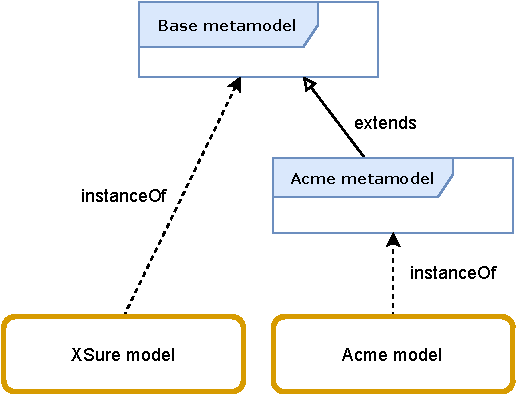
\includegraphics[width=0.7 \columnwidth]{Figures/MultilevelArchitecture.pdf}
    \caption{Multilevel architecture for the Process Challenge}
    \label{fig:MultilevelArchitecture}
\end{figure}

Also as our understanding, the use case analysis leads to identify two main modeling axis (as presented in figure \ref{fig:LinguisticAndOntologicInstantiation}):
\begin{itemize}
    \item the horizontal axis is characterized as the ontological instantiation axis, in the sense that the domain type definition (ProcessType as example) is referenced by an instance definition (Process, a.e). In our base  VirtualModel, each domain type definition is referenced by its instance definition, as developed in the section \ref{sec:ProcessEnactment}

\item the vertical axis is viewed as the linguistic instantiation, relative to the use of the FML language. The VirtualModel, defined as the core definition model, generates a model founded on the instantiation mechanism of the FML Language. This mechanism is the classical Object/Instance mechanism of the object languages but without any constraint on the referenced VirtualModel. The set of resulted instances comes from several VirtualModels 
from any abstraction level as detailed in section \ref{sec:AcmeSoftwareDevelopmentProcess}


\end{itemize}

\begin{figure}
    \centering
    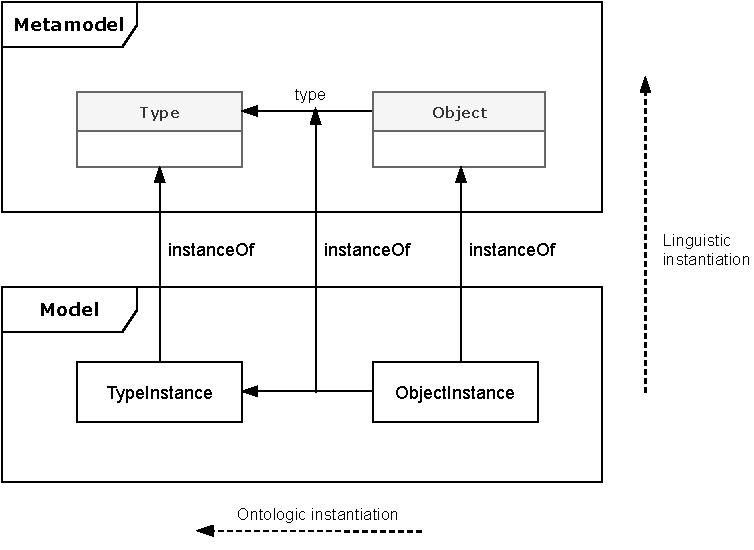
\includegraphics[width=1.0 \columnwidth]{Figures/Instantiation.pdf}
    \caption{Linguistic and ontologic instantiation}
    \label{fig:LinguisticAndOntologicInstantiation}
\end{figure}

Based on this approach, we organize our set of models as presented by the figure \ref{fig:MultilevelArchitecture}. The resulted multi-level architecture is organized as a set of VirtualModels. The first one is the core concepts model including the definition of Processes and Tasks. The second one, Acme VirtualModel, is extended from the previous model to integrate the Acme definitions. Our FML language defines the multiple inheritance concept between VirtualModels as illustrated in the section \ref{sec:AcmeSoftwareDevelopmentProcess}.

Finally as explained previously, the defined level for the Acme model and the XSure is the result of the instantiation of VirtualModels of different levels. In our approach this level can't be specialized or extended but all the other VirtualModels could be extended  by any concepts, as a new federated model. 



% il reste à décrire l'architecture générale des VirtualModels


~\\
~\\


\todo[inline]{quelles hypothèses supplémentaires ?}
%\todo[inline]{+ architecture de la modélisation (ce qui se trouve dans le ppt), le détail se retrouvera dans la section suivante}

